%\documentstyle[epsf,twocolumn]{jarticle}       %LaTeX2e仕様
%\documentclass[twocolumn]{jarticle}     %pLaTeX2e仕様(platex.exeの場合)
\documentclass[onecolumn]{ujarticle}   %pLaTeX2e仕様(uplatex.exeの場合)
%%%%%%%%%%%%%%%%%%%%%%%%%%%%%%%%%%%%%%%%%%%%%%%%%%%%%%%%%%%%%%
%%
%%  基本バージョン
%%
%%%%%%%%%%%%%%%%%%%%%%%%%%%%%%%%%%%%%%%%%%%%%%%%%%%%%%%%%%%%%%%%
\setlength{\topmargin}{-45pt}
%\setlength{\oddsidemargin}{0cm}
\setlength{\oddsidemargin}{-7.5mm}
%\setlength{\evensidemargin}{0cm}
\setlength{\textheight}{24.1cm}
%setlength{\textheight}{25cm}
\setlength{\textwidth}{17.4cm}
%\setlength{\textwidth}{172mm}
\setlength{\columnsep}{11mm}

%\kanjiskip=.07zw plus.5pt minus.5pt

% 【節が変わるごとに (1.1)(1.2) … (2.1)(2.2) と数式番号をつけるとき】
%\makeatletter
%\renewcommand{\theequation}{%
%\thesection.\arabic{equation}} %\@addtoreset{equation}{section}
%\makeatother

%\renewcommand{\arraystretch}{0.95} 行間の設定
%%%%%%%%%%%%%%%%%%%%%%%%%%%%%%%%%%%%%%%%%%%%%%%%%%%%%%%%
%\usepackage{graphicx}   %pLaTeX2e仕様(\documentstyle ->\documentclass)
\usepackage[dvipdfmx]{graphicx}
\usepackage{subcaption}
\usepackage{multirow}
\usepackage{amsmath}
\usepackage{url}
\usepackage[bb=boondox]{mathalfa}
\usepackage{listings}
\newcommand{\argmax}{\mathop{\rm arg~max}\limits}
\newcommand{\argmin}{\mathop{\rm arg~min}\limits}

\lstset{%
  language={Python},
  basicstyle={\small},%
  identifierstyle={\small},%
  commentstyle={\small\itshape},%
  keywordstyle={\small\bfseries},%
  ndkeywordstyle={\small},%
  stringstyle={\small\ttfamily},
  frame={tb},
  breaklines=true,
  columns=[l]{fullflexible},%
  numbers=left,%
  xrightmargin=0zw,%
  xleftmargin=3zw,%
  numberstyle={\scriptsize},%
  stepnumber=1,
  numbersep=1zw,%
  lineskip=-0.5ex%
}

%%%%%%%%%%%%%%%%%%%%%%%%%%%%%%%%%%%%%%%%%%%%%%%%%%%%%%%%
\begin{document}

	%bibtex用の設定
	%\bibliographystyle{ujarticle}
	\noindent

	\hspace{1em}
	2020 年 7 月 10 日
	ゼミ資料
	\hfill
	M2 寺内 光

	\vspace{2mm}

	\hrule

	\begin{center}
		{\Large \bf 進捗報告}
	\end{center}

	\hrule
	\vspace{3mm}

	% ‚ここから 文章 Start!
	\section{今週やったこと}
	\begin{itemize}{
    \item{TDGA の温度スケジューラのアップデート}
		\item{FastAutoAugmentへの TDGA の適用}
	}\end{itemize}
	\section{TDGA の温度スケジューラのアップデート}
  TDGA の温度スケジューラのアップデートをした.関数を渡す場合には漸化式の形で更新される仕様はそのままに(ちなみに漸化式を用いる場合,倍率 $\gamma$ は $0.8 \leq \gamma < 1$ がいいとされる \cite{SAschedule}),新たに初期温度と終了温度を指定して,現在の世代を $g_{\rm{now}}$, 終了世代を $g_{\rm{max}}$, 初期温度を $T_0$, 終了温度を $T_1$ として現在の温度 $T$ を以下のように設定できるようになった.これは一般的な焼きなまし法でよく用いられる指数スケジューラである.ナップサック問題での適切な動作を確認し,既にマスターに push 済み.

  \begin{eqnarray*}
    t = \frac{g_{\rm{now}}}{g_{\rm{max}}} \\ \\
    T = T_0^{1-t} * T_1^{t}
  \end{eqnarray*}

  この関数は $T_0 = 5$, $T_1 = 2$ のとき下のようなグラフになる.
  \begin{figure}[h]
		\begin{center}
			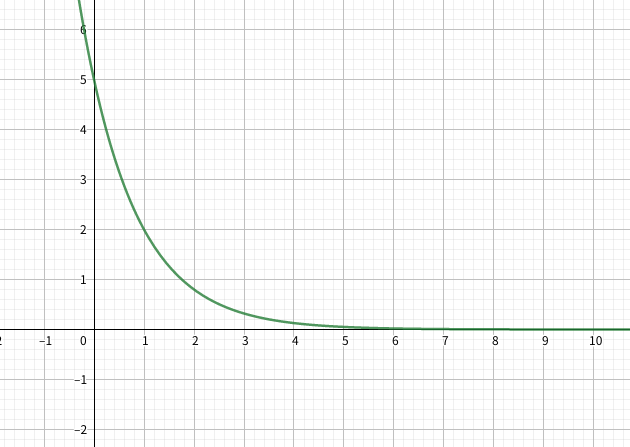
\includegraphics[width=0.7\columnwidth]{TGraph.png}
			\caption{初期温度と終了温度を定めた指数スケジューラ($T_0 = 5$, $T_1 = 2$)}
			\label{fig:variousmute}
		\end{center}
	\end{figure}


	\section{FastAutoAugmentへの TDGA の適用}
  FastAutoAugmentでの TDGA の動作が確認できた.10 個体で 100 世代進化させて 30時間程(評価回数がだいたい16000回).GAパートで24時間,子モデルの学習で6時間くらいの割合.
  現在の改良に関する調整検討項目としては,以下のようなものがある.

  \begin{itemize}
    \item{遺伝子表現}
    \item{個体数と世代数の調整}
    \item{突然変異の選択}
    \item{初期温度の選択,温度スケジューラの導入}
    \item{lossの最小化かaccの最大化か}
    \item{最終的にどの拡張を採用するか}
  \end{itemize}

  \subsection{遺伝子表現}
  ある拡張を使うか使わないかのビットエンコーディングと強度まで含めた整数値エンコーディングが考えられるが,1 世代に十分な個体数を確保するのが難しいので多様度を適切に計算するためにはビットエンコーディングが良さそう.

  \subsection{個体数と世代数の調整}
  エントロピー維持的な観点から言うと個体数の方を確保したい.それぞれのパラメータの増加に伴って実行時間は線形オーダーで増えるのでバランスを見ながら調整する.

  \subsection{突然変異(方法,確率)の選択}
  ビットエンコーディングはビット反転でいいとして,整数値エンコーディングのとき何を使うか.ランダムな整数値に変化させる or プラマイ1 の値に変化させる等.前者の方が局所解から抜け出せる性質を持っている一方,個体を悪化させる要因にもなりうる.突然変異確率も遷移させつつ.

  \subsection{初期温度の選択, 温度スケジューラの導入}
  平均エネルギーに対して温度パラメータはどれくらいの大きさが適切か(何か参考文献はありませんか).
  また,明示的に収束させる場合,温度スケジューラはどのようなものが良いのか,世代数はどれくらいが良いのか等.

  \subsection{lossの最小化かaccの最大化か}
  GA として最小化問題にするか最大化問題にするか.TDGA 的には accuracy の方が扱いやすそう? どれくらい個体間に差が出てくるかで変わってきそう.

  \subsection{最終的にどの拡張を採用するか}
  現在は 1 つの子モデルに対してランダムな初期値から 2 回探索をすることにより(元のベイズでのやり方),最良な拡張を2つ得ている.これを4つの子モデルに対して適用するため 8 つの拡張結果が得られることになる.時間の短縮的観点から言うと2回探索しているところを多様度も含めて最良のものを 2 つとってくるようにすると良さそう.


  来週は進化の過程も見つつ上記パラメータの調整をしていく.

	\section{来週のタスク}
	FastAutoAugment+TDGA(SGA) の調整しつつ 余裕があればRandAugmentを動かす(精度検証).

	% 参考文献リスト
	\bibliographystyle{unsrt}
	\bibliography{2020_07_10}
\end{document}
